% Copyright 2018-2020 Melvin Eloy Irizarry-Gelpí
\setcounter{chapter}{10}
\chapter{Diffraction}
%
In this experiment you will learn about diffraction of light from a laser due to a single slit.
%
\section{Preliminary}
%
When light passes through a double slit, an interference pattern is produced. The physical mechanism responsible for this is \textbf{diffraction}. The interference pattern arises as the combination of the diffraction pattern from each slit in the double slit.

You looked at interference patterns from a double slit in the previous experiment: A collection of dark and bright fringes. A diffraction pattern is similar, but has less structure (e.g. no ``internal'' fringes). For the interference pattern, you found that the distance between nearby \textbf{peaks} was almost constant and close to the theoretical value
\begin{equation}
    \Delta y \approx \frac{D \lambda}{d}
\end{equation}
Here $D$ is the longitudinal distance between the slit and the screen where the pattern appears, $\lambda$ is the wavelength of the laser light, and $d$ is the separation between the two slits. If the distance between nearby peaks is the same, then it follows that the distance $y_{n}$ from the central peak to the $n$-th peak is given by
\begin{equation}
    y_{n} \approx \frac{n D \lambda}{d}
\end{equation}
There is an analogous result for a diffraction pattern from a single slit. However, for a single slit there is no slit separation $d$, so instead the \textbf{slit width} $a$ plays a role:
\begin{equation}
    x_{n} \approx \frac{n D \lambda}{a}
\end{equation}
The interpretation is also different: $x_{n}$ is now the distance from the central peak to the $n$-th dark region (valley). In order to emphasize this subtle difference, I encourage you to use $y$ for distance from the center to a bright peak, and $x$ for distance from the center to a dark valley.
%
\subsection{Intensity}
%
Since the interference and diffraction patterns involve dark and bright regions, it is useful to measure the brightness. In your experiment this is done with a light intensity sensor. For practical purposes, light intensity is measured in units of percentage (\%). Dark regions have small percentage of intensity, and bright regions have large percentages. One observation about the intensity of the many bright regions in a pattern is that the intensity appears to change from peak to peak. For single slit diffraction there is a particular prediction for the ratio of the intensity of bright peaks. Let $I_{0}$ be the intensity of the central bright peak, $I_{1}$ be the intensity of the first bright peak, and $I_{2}$ be the intensity of the second bright peak. Then you expect that
\begin{align}
    \frac{I_{1}}{I_{0}} = 0.045 && \frac{I_{2}}{I_{0}} = 0.016
\end{align}
That is, the intensity of the first bright peak away from the center should be about 4.5\% the intensity of the central bright peak. Similarly, the intensity of the second bright peak away from the center should be about 1.6\% the intensity of the central bright peak. These relations should hold for bright peaks on both sides.
%
\section{Experiment}
%
The experiment consisted of collecting light intensity data for diffraction patterns from different single slits:
\begin{itemize}
    \item Single slit with $a = 0.08$ mm
    \item Single slit with $a = 0.04$ mm
    \item Single slit with $a = 0.16$ mm
\end{itemize}
For each single slit configuration you should have two runs, for consistency.
%
\section{Analysis}
%
The analysis for this experiment is very similar to the analysis in the previous experiment with the interference pattern. The main difference is that you need to find the position of dark valleys now, instead of bright peaks before.
%
\section{My Data}
%
For my data I used the \textbf{red laser}, so the wavelength value is $6.35 \times 10^{-4}$ mm. I also collected data for the $a = 0.02$ mm slit (runs 7 and 8).
%
\section{Your Data}
%
For your data you used the \textbf{green laser}, so the wavelength value is $5.32 \times 10^{-4}$ mm.
%
\newpage
\section{Your Report}
%
Your report should include the following:
\begin{itemize}
    \item A table like Table \ref{table.11.results.12} with the distance values for the $a = 0.08$ mm slit (either run 1 or run 2).
    \item A table like Table \ref{table.11.results.34} with the distance values for the $a = 0.04$ mm slit (either run 4 or run 4).
    \item A table like Table \ref{table.11.results.56} with the distance values for the $a = 0.16$ mm slit (either run 5 or run 6).
    \item A table like Table \ref{table.11.intensity.8} with the intensity ratios for the $a = 0.08$ mm slit (either run 1 or run 2).
    \item A table like Table \ref{table.11.intensity.4} with the intensity ratios for the $a = 0.04$ mm slit (either run 3 or run 4).
    \item A table like Table \ref{table.11.intensity.16} with the intensity ratios for the $a = 0.16$ mm slit (either run 5 or run 6).
    \item A chart like Figure \ref{figure.11.chart1} with the intensity profile for the $a = 0.08$ mm slit (either run 1 or run 2).
    \item A chart like Figure \ref{figure.11.chart2} with the intensity profile for the $a = 0.04$ mm slit (either run 3 or run 4).
    \item A chart like Figure \ref{figure.11.chart3} with the intensity profile for the $a = 0.16$ mm slit (either run 5 or run 6).
    \item Which diffraction slit yields the dark valleys that are closest to the central bright peak?
    \item Which diffraction slit yields the dark valleys that are farthest to the central bright peak?
\end{itemize}
%
\newpage
\section{Tables}
%
\begin{table}[ht!]
    \centering
    \begin{tabular}{|l|r|}
        \hline
        Feature & Position (mm) \\
        \hline
        Valley 3L & 50.08 \\
        Valley 2L & 57.32 \\
        Valley 1L & 65.11 \\
        \hline
        Peak 0C & 72.77 \\
        \hline
        Valley 1R & 79.8 \\
        Valley 2R & 87.29 \\
        Valley 3R & 94.61 \\
        \hline
    \end{tabular}
    \caption{Positions for Run 2 ($a = 0.08$ mm)}
    \label{table.11.pos.12}
\end{table}
%
\begin{table}[ht!]
    \centering
    \begin{tabular}{|l|r|}
        \hline
        Feature & Position (mm) \\
        \hline
        Valley 2L & 51.73 \\
        Valley 1L & 65.19 \\
        \hline
        Peak 0C & 81.15 \\
        \hline
        Valley 1R & 95.46 \\
        Valley 2R & 109.98 \\
        \hline
    \end{tabular}
    \caption{Positions for Run 4 ($a = 0.04$ mm)}
    \label{table.11.pos.34}
\end{table}
%
\begin{table}[ht!]
    \centering
    \begin{tabular}{|l|r|}
        \hline
        Feature & Position (mm) \\
        \hline
        Valley 3L & 66.8 \\
        Valley 2L & 70.57 \\
        Valley 1L & 74.34 \\
        \hline
        Peak 0C & 77.94 \\
        \hline
        Valley 1R & 81.66 \\
        Valley 2R & 85.43 \\
        Valley 3R & 89.24 \\
        \hline
    \end{tabular}
    \caption{Positions for Run 5 ($a = 0.16$ mm)}
    \label{table.11.pos.56}
\end{table}
%
\newpage
\begin{table}[ht!]
    \centering
    \begin{tabular}{|l|r|}
        \hline
        Difference & Distance (mm) \\
        \hline
        Valley 3L -- Peak 0C & $-22.69$ \\
        Valley 2L -- Peak 0C & $-15.45$ \\
        Valley 1L -- Peak 0C & $-7.66$ \\
        \hline
        Valley 1R -- Peak 0C & 7.03 \\
        Valley 2R -- Peak 0C & 14.52 \\
        Valley 3R -- Peak 0C & 21.84 \\
        \hline
    \end{tabular}
    \caption{Distances for Run 2 ($a = 0.08$ mm)}
    \label{tablel.11.dis.12}
\end{table}
%
\begin{table}[ht!]
    \centering
    \begin{tabular}{|l|r|}
        \hline
        Difference & Distance (mm) \\
        \hline
        Valley 2L -- Peak 0C & $-29.42$ \\
        Valley 1L -- Peak 0C & $-15.96$ \\
        \hline
        Valley 1R -- Peak 0C & 14.31 \\
        Valley 2R -- Peak 0C & 28.83 \\
        \hline
    \end{tabular}
    \caption{Distances for Run 4 ($a = 0.04$ mm)}
    \label{tablel.11.dis.34}
\end{table}
%
\begin{table}[ht!]
    \centering
    \begin{tabular}{|l|r|}
        \hline
        Difference & Distance (mm) \\
        \hline
        Valley 3L -- Peak 0C & $-11.14$ \\
        Valley 2L -- Peak 0C & $-7.37$ \\
        Valley 1L -- Peak 0C & $-3.6$ \\
        \hline
        Valley 1R -- Peak 0C & 3.72 \\
        Valley 2R -- Peak 0C & 7.49 \\
        Valley 3R -- Peak 0C & 11.3 \\
        \hline
    \end{tabular}
    \caption{Distances for Run 5 ($a = 0.16$ mm)}
    \label{tablel.11.dis.56}
\end{table}
%
\newpage
\begin{table}[ht!]
    \centering
    \begin{tabular}{|l|r|r|r|}
        \hline
        $n$ & Observed $x_{n}$ (mm) & Expected $x_{n}$ (mm) & P.D. (\%) \\
        \hline
        $-3$ & $-22.69$ & $-22.38$ & 1.37 \\
        $-2$ & $-15.45$ & $-14.92$ & 3.53 \\
        $-1$ & $-7.66$ & $-7.46$ & 2.66 \\
        \hline
        $+1$ & 7.03 & 7.46 & $-5.78$ \\
        $+2$ & 14.52 & 14.92 & $-2.70$ \\
        $+3$ & 21.84 & 22.38 & $-2.43$ \\
        \hline
    \end{tabular}
    \caption{Results for Run 2 ($a = 0.08$ mm)}
    \label{table.11.results.12}
\end{table}
%
\begin{table}[ht!]
    \centering
    \begin{tabular}{|l|r|r|r|}
        \hline
        $n$ & Observed $x_{n}$ (mm) & Expected $x_{n}$ (mm) & P.D. (\%) \\
        \hline
        $-2$ & $-29.42$ & $-29.85$ & $-1.42$ \\
        $-1$ & $-15.96$ & $-14.92$ & 6.95 \\
        \hline
        $+1$ & 14.31 & 14.92 & $-4.10$ \\
        $+2$ & 28.83 & 29.85 & $-3.40$ \\
        \hline
    \end{tabular}
    \caption{Results for Run 4 ($a = 0.04$ mm)}
    \label{table.11.results.34}
\end{table}
%
\begin{table}[ht!]
    \centering
    \begin{tabular}{|l|r|r|r|}
        \hline
        $n$ & Observed $x_{n}$ (mm) & Expected $x_{n}$ (mm) & P.D. (\%) \\
        \hline
        $-3$ & $-11.14$ & $-11.19$ & $-0.46$ \\
        $-2$ & $-7.37$ & $-7.46$ & $-1.22$ \\
        $-1$ & $-3.6$ & $-3.73$ & $-3.50$ \\
        \hline
        $+1$ & 3.72 & 3.73 & $-0.28$ \\
        $+2$ & 7.49 & 7.46 & 0.39 \\
        $+3$ & 11.3 & 11.19 & 0.97 \\
        \hline
    \end{tabular}
    \caption{Results for Run 5 ($a = 0.16$ mm)}
    \label{table.11.results.56}
\end{table}
%
\newpage
\begin{table}[ht!]
    \centering
    \begin{tabular}{|l|r|}
        \hline
        Ratio & Value \\
        \hline
        $I_{\text{3L}} / I_{\text{0C}}$ & 0.017 \\
        $I_{\text{2L}} / I_{\text{0C}}$ & 0.025 \\
        $I_{\text{1L}} / I_{\text{0C}}$ & 0.055 \\
        \hline
        $I_{\text{1R}} / I_{\text{0C}}$ & 0.065 \\
        $I_{\text{2R}} / I_{\text{0C}}$ & 0.031 \\
        $I_{\text{3R}} / I_{\text{0C}}$ & 0.021 \\
        \hline
    \end{tabular}
    \caption{Intensity ratios for Run 2 ($a = 0.08$ mm)}
    \label{table.11.intensity.8}
\end{table}
%
\begin{table}[ht!]
    \centering
    \begin{tabular}{|l|r|}
        \hline
        Ratio & Value \\
        \hline
        $I_{\text{1L}} / I_{\text{0C}}$ & 0.086 \\
        \hline
        $I_{\text{1R}} / I_{\text{0C}}$ & 0.099 \\
        \hline
    \end{tabular}
    \caption{Intensity ratios for Run 4 ($a = 0.04$ mm)}
    \label{table.11.intensity.4}
\end{table}
%
\begin{table}[ht!]
    \centering
    \begin{tabular}{|l|r|}
        \hline
        Ratio & Value \\
        \hline
        $I_{\text{3L}} / I_{\text{0C}}$ & 0.010 \\
        $I_{\text{2L}} / I_{\text{0C}}$ & 0.020 \\
        $I_{\text{1L}} / I_{\text{0C}}$ & 0.051 \\
        \hline
        $I_{\text{1R}} / I_{\text{0C}}$ & 0.059 \\
        $I_{\text{2R}} / I_{\text{0C}}$ & 0.025 \\
        $I_{\text{3L}} / I_{\text{0C}}$ & 0.014 \\
        \hline
    \end{tabular}
    \caption{Intensity ratios for Run 5 ($a = 0.16$ mm)}
    \label{table.11.intensity.16}
\end{table}
%
\FloatBarrier
\newpage
\section{Figures}
%
\begin{figure}[ht!]
	\centering
	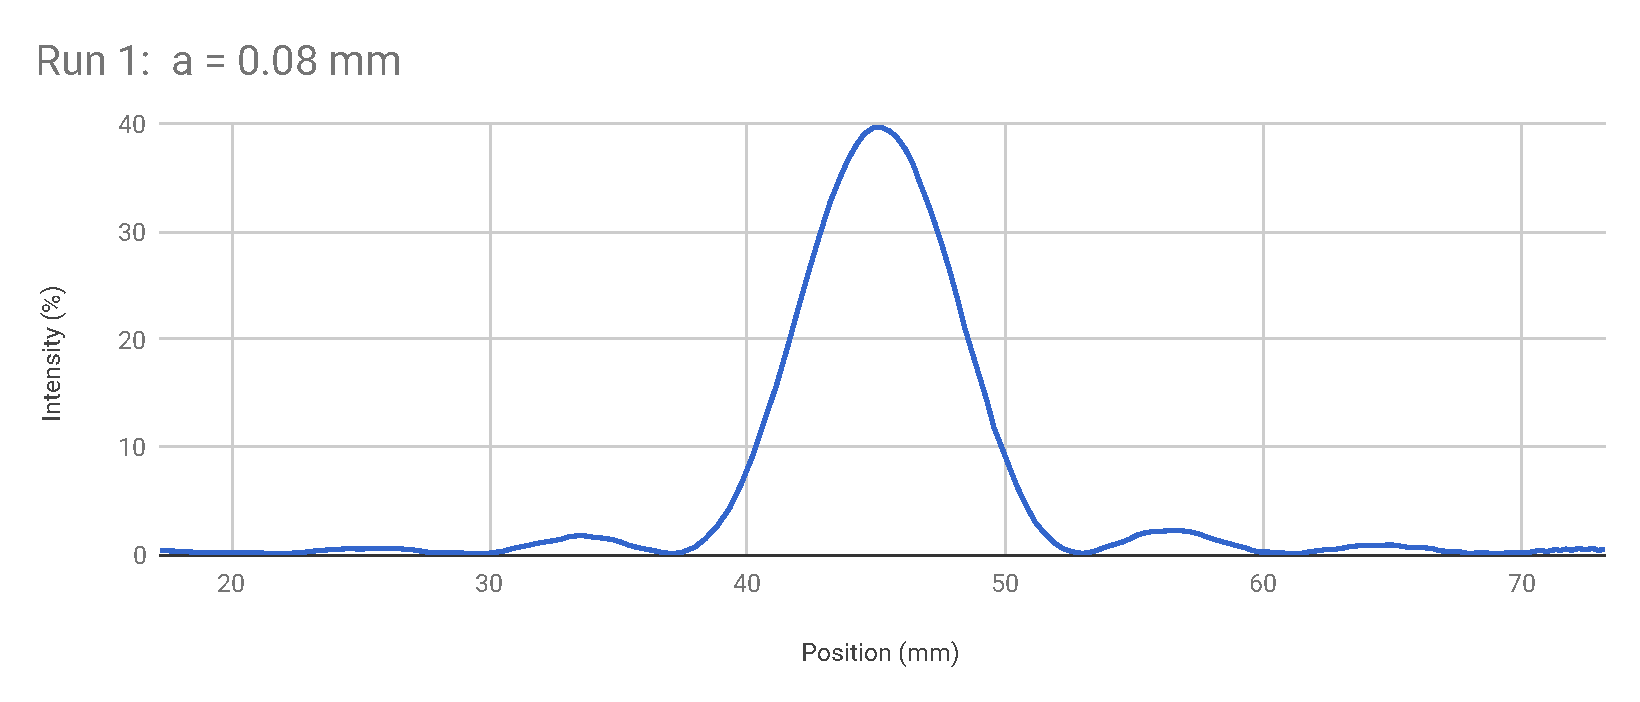
\includegraphics[scale=0.74]{image/11-diffraction/chart1.pdf}
	\caption{Intensity for diffraction pattern with $a = 0.08$ mm.}
	\label{figure.11.chart1}
\end{figure}
%
\begin{figure}[ht!]
	\centering
	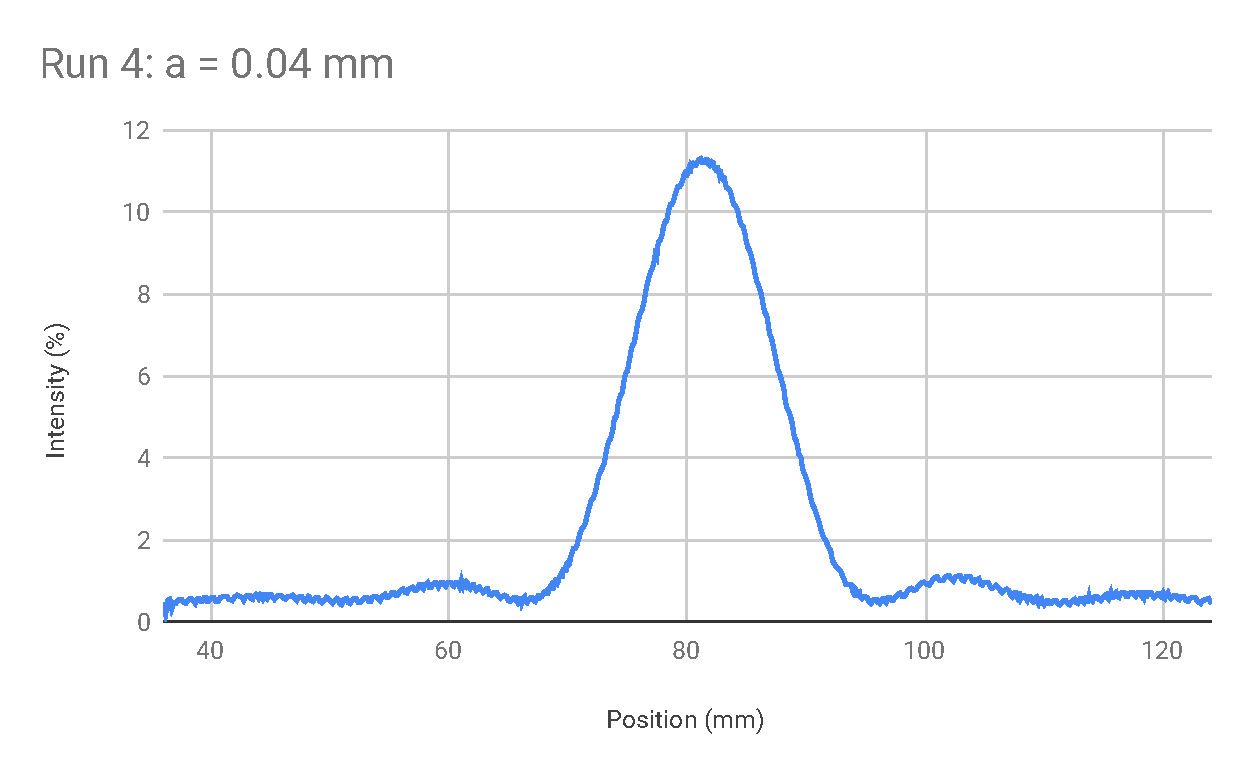
\includegraphics[scale=0.74]{image/11-diffraction/chart2.pdf}
	\caption{Intensity for diffraction pattern with $a = 0.04$ mm.}
	\label{figure.11.chart2}
\end{figure}
%
\begin{figure}[ht!]
	\centering
	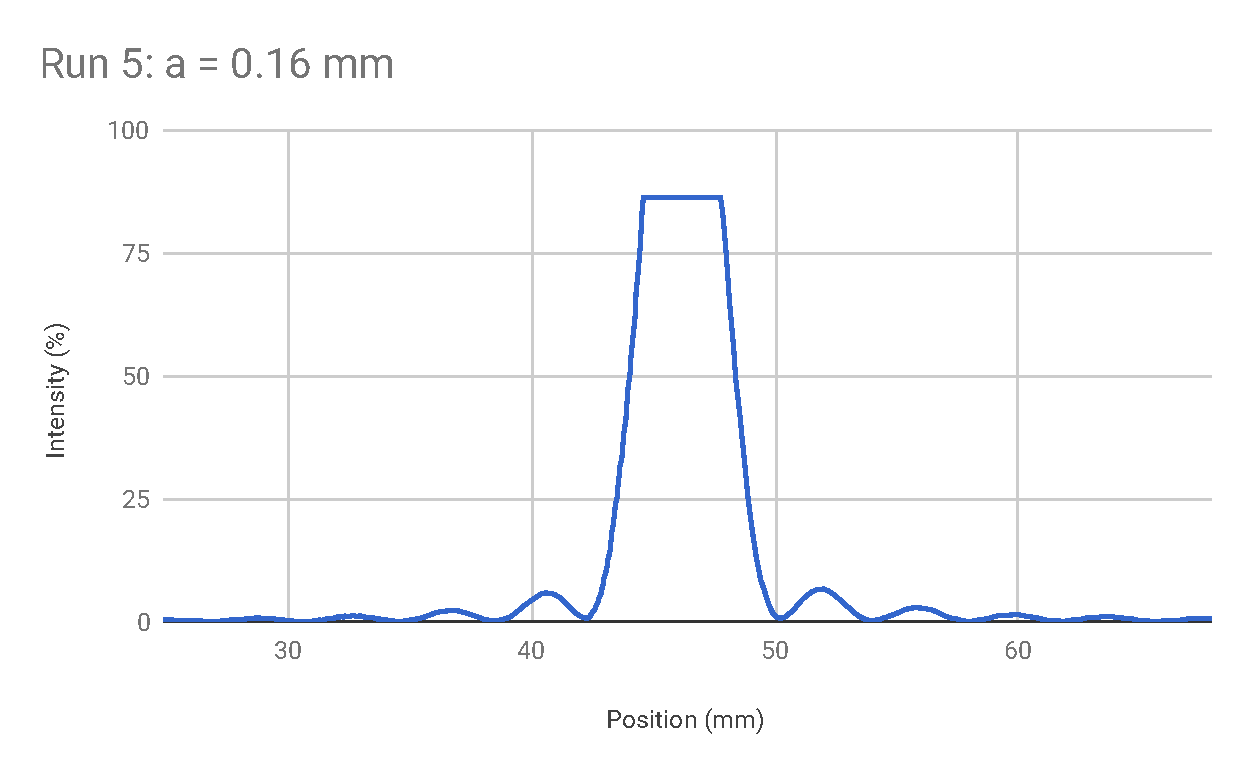
\includegraphics[scale=0.74]{image/11-diffraction/chart3.pdf}
	\caption{Intensity for diffraction pattern with $a = 0.16$ mm.}
	\label{figure.11.chart3}
\end{figure}
%